% pgfplots chart for Table VII — \usepackage{pgfplots}\pgfplotsset{compat=1.18}
\begin{figure}[t]\centering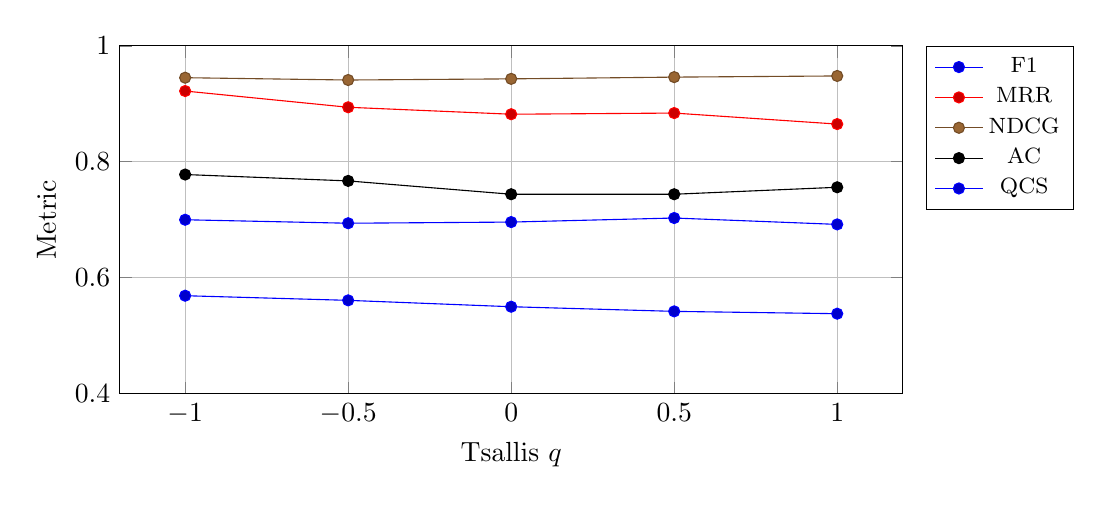
\begin{tikzpicture}
\begin{axis}[width=.95\linewidth,height=6cm,xlabel={Tsallis $q$},ylabel={Metric},
  legend pos=outer north east,grid=both,xtick={-1,-0.5,0,0.5,1},ymin=0.4,ymax=1.0,
  legend style={font=\footnotesize}]
\addplot+[mark=*] coordinates {(-1,0.700) (-0.5,0.694) (0,0.696) (0.5,0.703) (1,0.692)}; \addlegendentry{F1}
\addplot+[mark=*] coordinates {(-1,0.922) (-0.5,0.894) (0,0.882) (0.5,0.884) (1,0.865)}; \addlegendentry{MRR}
\addplot+[mark=*] coordinates {(-1,0.945) (-0.5,0.941) (0,0.943) (0.5,0.946) (1,0.948)}; \addlegendentry{NDCG}
\addplot+[mark=*] coordinates {(-1,0.778) (-0.5,0.767) (0,0.744) (0.5,0.744) (1,0.756)}; \addlegendentry{AC}
\addplot+[mark=*] coordinates {(-1,0.569) (-0.5,0.561) (0,0.550) (0.5,0.542) (1,0.538)}; \addlegendentry{QCS}
\end{axis}\end{tikzpicture}
\caption{Effect of the Tsallis $q$ on retrieval metrics (averaged across all corpora).}
\label{fig:qsweep}\end{figure}